\documentclass[aspectratio=169,xcolor=dvipsnames]{beamer}
% 1. Definir el color ANTES de llamar al tema SimplePlus
\usepackage{xcolor}
\definecolor{nyugray}{RGB}{128,128,128}
\usetheme{SimplePlus}
\definecolor{UnalGreen}{RGB}{0,153,51}
\usepackage[utf8]{inputenc}
\usepackage[spanish]{babel}
\usepackage{hyperref}
\usepackage{graphicx}
\usepackage{booktabs}
\usepackage{tikz}
\usepackage{pgfplots}
% NOTA: no se declara \pgfplotsset{compat=...} a propósito (ver convenciones del curso)
\usetikzlibrary{positioning, arrows.meta, babel}
\usepackage[skip=5pt]{caption}
\captionsetup{justification=justified, font=small}
\usefonttheme{professionalfonts}

% ----- PLACEHOLDER PARA IMÁGENES EXTERNAS -----
\newcommand{\imgwarning}[2][0.8]{%
	\begin{center}
		\fcolorbox{nyugray}{gray!8}{%
			\parbox[c][3.2cm][c]{#1\textwidth}{\centering\small\textcolor{nyugray}{%
					[\,Insertar imagen: #2\,]}}%
		}
	\end{center}
}

\title{Fundamentos de Mecánica -- Taller}
\subtitle{Sesión 3: Cinemática 2D}
\titlegraphic{%
	\vspace*{-0.3cm}%
	\IfFileExists{imagenes/universidad-nacional-de-colombia-sede-bogota-seeklogo.png}{%
		\includegraphics[width=2.2cm]{imagenes/universidad-nacional-de-colombia-sede-bogota-seeklogo.png}%
	}{%
		\IfFileExists{universidad-nacional-de-colombia-sede-bogota-seeklogo.png}{%
			
\includegraphics[width=2.2cm]{universidad-nacional-de-colombia-sede-bogota-seeklogo.png}%
		}{}%
	}%
	\hspace{1.0cm}%
	\IfFileExists{logoMIAI_white.png}{%
		
\includegraphics[width=4.0cm]{logoMIAI_white.png}%
	}{%
		\IfFileExists{imagenes/logoMIAI_white.png}{%
			\includegraphics[width=4.0cm]{imagenes/logoMIAI_white.png}%
		}{}%
	}%
}
\author{Miguel Andrés Perdomo Gutiérrez}
\institute{%
	Auxiliar Docente | M.Sc. en Ciencias -- Física\\
	Universidad Nacional de Colombia -- Sede Bogotá
}
\date{18 de septiembre de 2026}

\begin{document}
	
	% ============================================================
	% SLIDE 1: PORTADA
	% ============================================================
	\begin{frame}
		\titlepage
	\end{frame}
	
	% ============================================================
	% SLIDE 2: AGENDA DE LA SESIÓN
	% ============================================================
	\begin{frame}{Agenda de la Sesión}
		\centering
		\begin{tikzpicture}[
			box/.style={rectangle, rounded corners, draw=UnalGreen, thick, fill=UnalGreen!10,
				minimum width=2.4cm, minimum height=1.7cm, align=center, font=\small},
			arr/.style={-{Latex[length=2mm]}, thick, UnalGreen}
			]
			\node[box] (b1) {Primer\\Quiz\\\textbf{20 min}};
			\node[box, right=0.5cm of b1] (b2) {Grupos de\\trabajo\\\textbf{5 min}};
			\node[box, right=0.5cm of b2] (b3) {Cinemática 2D:\\Tiro parabólico\\\textbf{60 min}};
			\node[box, right=0.5cm of b3] (b4) {Preguntas\\y dudas\\\textbf{10 min}};
			\draw[arr] (b1) -- (b2);
			\draw[arr] (b2) -- (b3);
			\draw[arr] (b3) -- (b4);
		\end{tikzpicture}
		
		\vspace{0.5cm}
		\begin{itemize}
			\item Duración total: \textbf{2 horas} (Viernes 09:00--11:00, Edificio 401, Salón 202).
			\item Primera parte: sustentación en tablero del Taller 2 (Cinemática 1D y Graficación).
			\item Segunda parte: extensión a dos dimensiones -- movimiento de proyectiles.
		\end{itemize}
	\end{frame}

	
	% ============================================================
	% SLIDE 4: TALLER 2 -- PROBLEMA 2 (DERIVACIÓN)
	% ============================================================
	\begin{frame}{Taller 2 -- Problema 2: La ecuación sin tiempo}
		\small
		\textbf{Partimos de:}
		\[
		x(t) = \tfrac{1}{2}a_x t^2 + v_{0x}t + x_0
		\qquad\qquad
		v_x(t) = v_{0x} + a_x t
		\]
		
		\textbf{Paso 1.} Despejamos $t$ de la segunda ecuación:
		\[
		t = \frac{v_x - v_{0x}}{a_x}
		\]
		
		\textbf{Paso 2.} Sustituimos en la primera y agrupamos $x - x_0$:
		\[
		x - x_0 = \frac{1}{2}a_x\left(\frac{v_x - v_{0x}}{a_x}\right)^{2}
		+ v_{0x}\left(\frac{v_x - v_{0x}}{a_x}\right)
		= \frac{(v_x-v_{0x})^2}{2a_x} + \frac{v_{0x}(v_x-v_{0x})}{a_x}
		\]
		
		\textbf{Paso 3.} Multiplicamos todo por $2a_x$:
		\[
		2a_x(x-x_0) = (v_x-v_{0x})^2 + 2v_{0x}(v_x-v_{0x})
		\]
	\end{frame}
	
	% ============================================================
	% SLIDE 5: TALLER 2 -- PROBLEMA 2 (CIERRE)
	% ============================================================
	\begin{frame}{Taller 2 -- Problema 2: Cierre algebraico}
		\small
		\textbf{Paso 4.} Expandimos ambos términos:
		\[
		(v_x-v_{0x})^2 = v_x^2 - 2v_xv_{0x} + v_{0x}^2
		\qquad
		2v_{0x}(v_x-v_{0x}) = 2v_{0x}v_x - 2v_{0x}^2
		\]
		
		\textbf{Paso 5.} Sumamos. Los términos cruzados se cancelan:
		\[
		v_x^2 \underbrace{- 2v_xv_{0x} + 2v_{0x}v_x}_{=\,0} + \underbrace{v_{0x}^2 - 2v_{0x}^2}_{=\,-v_{0x}^2}
		\;=\; v_x^2 - v_{0x}^2
		\]
		
		\vspace{0.2cm}
		\begin{exampleblock}{Resultado}
			\centering
			\Large $v_x^2 = v_{0x}^2 + 2a_x(x-x_0)$
		\end{exampleblock}
		
		\vspace{0.2cm}
		\begin{center}
			\small \textbf{¿Para qué sirve?} Relaciona velocidad y posición \textbf{sin necesidad de conocer $t$}.
			Es la herramienta natural cuando el problema no menciona tiempos.
		\end{center}
	\end{frame}
	
	% ============================================================
	% SLIDE 6: INCISO -- ¿QUÉ HACE BUENA UNA GRÁFICA?
	% =====================================
	
		% ============================================================
	% SLIDE 6: LOS DATOS
	% ============================================================
	\begin{frame}{Los datos: volumen de un gas vs.\ temperatura}
		\begin{center}
			\footnotesize
			\begin{tabular}{lccccccccc}
				\toprule
				$T$ ($^\circ$C) & 62.3 & 68.6 & 81.4 & 87.4 & 98.6 & 104.5 & 116.9 & 121.2 & 135.0 \\
				\midrule
				$V$ (cm$^3$) & 27073 & 28492 & 29300 & 29200 & 30849 & 31500 & 32100 & 32000 & 33500 \\
				\bottomrule
			\end{tabular}
		\end{center}
		
		\vspace{0.4cm}
		\begin{center}
			\small
			Los mismos datos se graficaron de tres maneras distintas.
			Observen cada panel y decidan cuál usarían en un informe y por qué.
		\end{center}
	\end{frame}
	
	% ============================================================
	% SLIDE 7: PANEL (a)
	% ============================================================
	\begin{frame}{Panel (a)}
		\begin{center}
			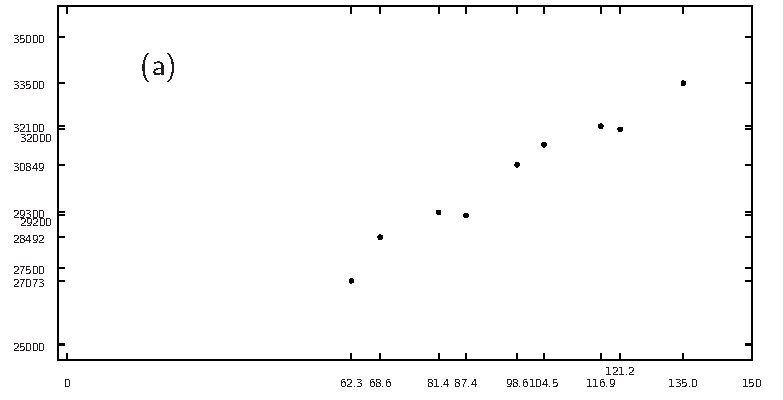
\includegraphics[width=\textwidth,height=0.85\textheight,keepaspectratio]{figura1.pdf}
		\end{center}
	\end{frame}
	
	% ============================================================
	% SLIDE 8: PANELES (b) Y (c)
	% ============================================================
	\begin{frame}{Paneles (b) y (c)}
		\begin{center}
			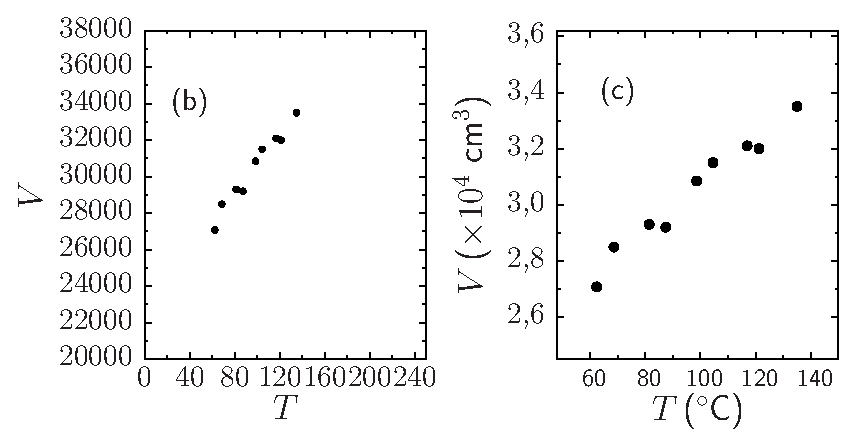
\includegraphics[width=\textwidth,height=0.85\textheight,keepaspectratio]{figura2.pdf}
		\end{center}
	\end{frame}
	% ============================================================
	% SLIDE 9: ¿CÓMO LES FUE CON LA GRAFICACIÓN?
	% ============================================================
	\begin{frame}{La parte opcional: midiendo $g$}
		\begin{columns}[T]
			\begin{column}{0.5\textwidth}
				\small
				La idea de Galileo: si
				\[
				h = \tfrac{1}{2}g\,t^2
				\]
				entonces al graficar $h$ contra $t^2$ (\textbf{no} contra $t$) se obtiene una \textbf{recta}
				de pendiente $m = g/2$.
				
				\vspace{0.25cm}
				\[
				g_{\text{exp}} = 2 \times m
				\]
				
				\vspace{0.25cm}
				\textcolor{UnalGreen}{\textbf{¿Quiénes lo intentaron?}}
				\begin{itemize}\small
					\item ¿Qué valor de $g$ obtuvieron?
					\item ¿Los puntos quedaron alineados?
				\end{itemize}
			\end{column}
			\begin{column}{0.5\textwidth}
				\begin{center}
					\begin{tikzpicture}
						\begin{axis}[width=6.0cm, height=4.6cm,
							xlabel={$t^2$ (s$^2$)}, ylabel={$h$ (m)},
							xmin=0, xmax=2.2, ymin=0, ymax=11,
							xtick={0,0.5,1,1.5,2}, ytick={0,2,4,6,8,10},
							grid=both, grid style={gray!30, thin}]
							\addplot[only marks, mark=*, mark size=1.8pt, UnalGreen]
							coordinates {(0.408,2) (0.816,4) (1.224,6) (1.633,8) (2.041,10)};
							\addplot[domain=0:2.2, samples=2, thick, red!70!black, dashed] {4.9*x};
						\end{axis}
					\end{tikzpicture}
				\end{center}
				\vspace{-0.2cm}
				\begin{center}
					\scriptsize Pendiente $m \approx 4.9 \Rightarrow g \approx 9.8$ m/s$^2$
				\end{center}
			\end{column}
		\end{columns}
	\end{frame}
	
	% ============================================================
	% SLIDE 10: DE 1D A 2D
	% ============================================================
	\begin{frame}{De una a dos dimensiones}
		\begin{block}{La idea central}
			\centering
			Un movimiento en el plano es \textbf{dos movimientos 1D independientes}, uno en $x$ y otro en $y$,
			que ocurren \textbf{al mismo tiempo}.
		\end{block}
		
		\vspace{0.3cm}
		\begin{columns}[T]
			\begin{column}{0.48\textwidth}
				\textbf{Posición y velocidad:}
				\[
				\vec{r}(t) = x(t)\,\hat{\imath} + y(t)\,\hat{\jmath}
				\]
				\[
				\vec{v}(t) = v_x(t)\,\hat{\imath} + v_y(t)\,\hat{\jmath}
				\]
			\end{column}
			\begin{column}{0.48\textwidth}
				\textbf{En un proyectil:}
				\[
				\vec{a}(t) = -g\,\hat{\jmath}
				\]
				\small La aceleración \textbf{solo} tiene componente vertical.
				En $x$ no hay aceleración.
			\end{column}
		\end{columns}
		
		\vspace{0.35cm}
		\begin{exampleblock}{Consecuencia inmediata}
			\centering
			En $x$: movimiento \textbf{uniforme} \qquad$\cdot$\qquad En $y$: movimiento \textbf{uniformemente acelerado}
		\end{exampleblock}
	\end{frame}
	
	% ============================================================
	% SLIDE 11: TIRO PARABÓLICO -- DESCOMPOSICIÓN
	% ============================================================
	% ============================================================
% SLIDE 11: TIRO PARABÓLICO -- DESCOMPOSICIÓN
% ============================================================
\begin{frame}{Tiro parabólico: descomposición de la velocidad}
	\begin{center}
		\begin{tikzpicture}[scale=1.05, every node/.style={font=\normalsize}]
			% Trayectoria
			\draw[thick, UnalGreen, domain=0:8, samples=100, smooth]
			plot (\x, {0.55*\x - 0.0688*\x*\x});
			
			% Ejes
			\draw[-{Latex[length=3mm]}, thick] (-0.4,0) -- (9.2,0) node[right, font=\large] {$x$};
			\draw[-{Latex[length=3mm]}, thick] (0,-0.5) -- (0,2.6) node[above, font=\large] {$y$};
			
			% Vector inicial y componentes
			\draw[-{Latex[length=3mm]}, very thick, red!75!black] (0,0) -- (1.7,0.94)
			node[midway, above left, font=\large] {$\vec{v}_0$};
			\draw[-{Latex[length=2.5mm]}, thick, dashed, nyugray] (0,0) -- (1.7,0)
			node[midway, below, font=\large] {$v_{0x}$};
			\draw[-{Latex[length=2.5mm]}, thick, dashed, nyugray] (1.7,0) -- (1.7,0.94)
			node[midway, right, font=\large] {$v_{0y}$};
			
			% Ángulo
			\draw[thick] (0.65,0) arc (0:29:0.65) node[midway, right, font=\large] {$\theta$};
			
			% Vector en el vértice
			\draw[-{Latex[length=3mm]}, very thick, red!75!black] (4,1.1) -- (5.5,1.1)
			node[midway, above, font=\large] {$v_x = v_{0x}$};
			\fill (4,1.1) circle (2.2pt);
		\end{tikzpicture}
	\end{center}
	
	\vspace{0.25cm}
	\begin{center}
		\large $v_{0x} = v_0\cos\theta$ \qquad\qquad $v_{0y} = v_0\sin\theta$
	\end{center}
	
	\vspace{0.2cm}
	\begin{center}
		\large \textcolor{UnalGreen}{\textbf{Note:}} la componente horizontal \textbf{nunca cambia};
		la vertical se anula en el vértice y luego se invierte.
	\end{center}
\end{frame}
	
	% ============================================================
	% SLIDE 12: LAS ECUACIONES
	% ============================================================
	\begin{frame}{Las ecuaciones del movimiento parabólico}
		\begin{columns}[T]
			\begin{column}{0.48\textwidth}
				\begin{block}{Eje horizontal ($a_x = 0$)}
					\[
					v_x(t) = v_{0x} = \text{cte}
					\]
					\[
					x(t) = v_{0x}\,t
					\]
				\end{block}
			\end{column}
			\begin{column}{0.48\textwidth}
				\begin{block}{Eje vertical ($a_y = -g$)}
					\[
					v_y(t) = -g\,t + v_{0y}
					\]
					\[
					y(t) = -\tfrac{1}{2}g\,t^2 + v_{0y}\,t
					\]
				\end{block}
			\end{column}
		\end{columns}
		
		\vspace{0.35cm}
		\begin{exampleblock}{¿Por qué la trayectoria es una parábola?}
			Despejamos $t = x/v_{0x}$ de la ecuación horizontal y sustituimos en la vertical:
			\[
			y = -\frac{g}{2}\left(\frac{x}{v_{0x}}\right)^{2} + v_{0y}\left(\frac{x}{v_{0x}}\right)
			\]
			\centering
			\small Es de la forma $y = Ax^2 + Bx$: \textbf{una parábola}.
		\end{exampleblock}
	\end{frame}
	
	% ============================================================
	% SLIDE 13: ALTURA MÁXIMA
	% ============================================================
	\begin{frame}{Altura máxima}
		\small
		\textbf{Condición:} en el punto más alto, la velocidad vertical se anula.
		\[
		v_y(t_h) = 0 \quad\Longrightarrow\quad -g\,t_h + v_{0y} = 0
		\quad\Longrightarrow\quad t_h = \frac{v_{0y}}{g}
		\]
		
		\vspace{0.15cm}
		\textbf{Sustituimos $t_h$ en $y(t)$:}
		\[
		h = y(t_h) = -\frac{g}{2}\left(\frac{v_{0y}}{g}\right)^{2} + v_{0y}\left(\frac{v_{0y}}{g}\right)
		= -\frac{v_{0y}^{2}}{2g} + \frac{v_{0y}^{2}}{g}
		\]
		
		\vspace{0.1cm}
		\begin{exampleblock}{}
			\centering
			\Large $h = \dfrac{v_{0y}^{2}}{2g} = \dfrac{v_{0}^{2}\sin^{2}\theta}{2g}$
		\end{exampleblock}
		
		\vspace{0.1cm}
		\begin{center}
			\small La altura máxima depende \textbf{solo} de la componente vertical de la velocidad inicial.
		\end{center}
	\end{frame}
	
	% ============================================================
	% SLIDE 14: RANGO
	% ============================================================
	\begin{frame}{Rango (alcance horizontal)}
		\small
		\textbf{Condición:} el proyectil vuelve al nivel de lanzamiento, $y = 0$.
		Por simetría de la parábola, el tiempo total es el doble del tiempo de subida:
		\[
		t_R = 2\,t_h = \frac{2v_{0y}}{g}
		\]
		
		\vspace{0.15cm}
		\textbf{Sustituimos en $x(t) = v_{0x}t$:}
		\[
		R = v_{0x}\left(\frac{2v_{0y}}{g}\right) = \frac{2\,v_{0x}v_{0y}}{g}
		\]
		
		\vspace{0.1cm}
		\textbf{En términos de $v_0$ y $\theta$}, usando $\sin 2\theta = 2\sin\theta\cos\theta$:
		\[
		R = \frac{2v_0^{2}\sin\theta\cos\theta}{g}
		\]
		
		\begin{exampleblock}{}
			\centering
			\Large $R = \dfrac{v_0^{2}\,\sin 2\theta}{g}$
		\end{exampleblock}
	\end{frame}
	
	% ============================================================
	% SLIDE 15: ÁNGULO DE MÁXIMO ALCANCE
	% ============================================================
	% ============================================================
% SLIDE 15: ÁNGULO DE MÁXIMO ALCANCE
% ============================================================
\begin{frame}{¿Qué ángulo da el mayor alcance?}
	\begin{columns}[T]
		\begin{column}{0.54\textwidth}
			\begin{center}
				\begin{tikzpicture}
					\begin{axis}[width=7.0cm, height=5.4cm,
						xlabel={$x$ (m)}, ylabel={$y$ (m)},
						xlabel style={yshift=2pt},
						ylabel style={yshift=-2pt},
						xmin=0, xmax=62, ymin=0, ymax=32,
						xtick={0,20,40,60}, ytick={0,10,20,30},
						grid=both, grid style={gray!25, thin},
						legend style={font=\scriptsize, at={(0.98,0.98)},
							anchor=north east, draw=none, fill=none, row sep=1pt}]
						
						% R = 24^2 * sin(2θ) / 9.8
						\addplot[domain=0:29.39, samples=80, thick, orange!85!black]
						{x*tan(15) - 9.8*x^2/(2*24^2*(cos(15))^2)};
						\addlegendentry{$\theta = 15^\circ$}
						
						\addplot[domain=0:50.91, samples=80, thick, UnalGreen]
						{x*tan(30) - 9.8*x^2/(2*24^2*(cos(30))^2)};
						\addlegendentry{$\theta = 30^\circ$}
						
						\addplot[domain=0:58.78, samples=80, thick, red!75!black]
						{x*tan(45) - 9.8*x^2/(2*24^2*(cos(45))^2)};
						\addlegendentry{$\theta = 45^\circ$}
						
						\addplot[domain=0:50.91, samples=80, thick, blue!65!black]
						{x*tan(60) - 9.8*x^2/(2*24^2*(cos(60))^2)};
						\addlegendentry{$\theta = 60^\circ$}
						
						\addplot[domain=0:29.39, samples=80, thick, violet]
						{x*tan(75) - 9.8*x^2/(2*24^2*(cos(75))^2)};
						\addlegendentry{$\theta = 75^\circ$}
					\end{axis}
				\end{tikzpicture}
			\end{center}
			\vspace{-0.15cm}
			\begin{center}\normalsize $v_0 = 24$ m/s\end{center}
		\end{column}
		\begin{column}{0.44\textwidth}
			\small
			El rango es máximo cuando $\sin 2\theta$ es máximo:
			\[
			\sin 2\theta_m = 1 \;\Longrightarrow\; 2\theta_m = 90^\circ
			\]
			\begin{exampleblock}{}
				\centering
				\Large \textcolor{red!75!black}{$\theta_m = 45^\circ$}
			\end{exampleblock}
			
			\vspace{0.25cm}
			\textbf{Además:} $15^\circ$ y $75^\circ$ dan \textbf{el mismo alcance};
			$30^\circ$ y $60^\circ$ también.
			
			\vspace{0.15cm}
			\small ¿Por qué? Porque $\sin(2\cdot 15^\circ) = \sin 30^\circ$
			y $\sin(2\cdot 75^\circ) = \sin 150^\circ$, y ambos valen lo mismo.
			
			\vspace{0.15cm}
			\textit{En general, $\theta$ y $90^\circ - \theta$ son ángulos complementarios con igual rango.}
		\end{column}
	\end{columns}
\end{frame}
	
	% ============================================================
	% SLIDE 16: INDEPENDENCIA DE LOS MOVIMIENTOS
	% ============================================================
	% ============================================================
% SLIDE 16: INDEPENDENCIA DE LOS MOVIMIENTOS
% ============================================================
\begin{frame}{Independencia de los movimientos}
	\begin{columns}[T]
		\begin{column}{0.5\textwidth}
			\begin{block}{El experimento}
				Dos pelotas se sueltan simultáneamente: una cae verticalmente, la otra sale
				disparada en horizontal.
				
				\vspace{0.25cm}
				\centering
				\textcolor{UnalGreen}{\textbf{¿Cuál llega primero al suelo?}}
			\end{block}
			
			\vspace{0.3cm}
			\small
			La respuesta: \textbf{llegan al mismo tiempo}.
			
			\vspace{0.15cm}
			El movimiento horizontal \textbf{no afecta} al vertical. La caída está gobernada
			únicamente por
			\[
			y(t) = -\tfrac{1}{2}g t^2 + y_0
			\]
			que no contiene ninguna información sobre $v_{0x}$.
		\end{column}
		\begin{column}{0.48\textwidth}
			\begin{center}
				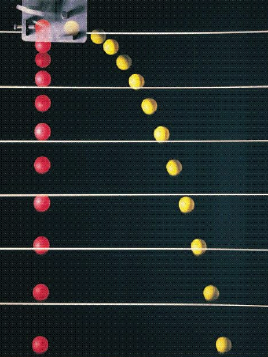
\includegraphics[width=\textwidth,height=0.75\textheight,keepaspectratio]{figura3.png}
			\end{center}
		\end{column}
	\end{columns}
\end{frame}
	% ============================================================
	% SLIDE 17: EJEMPLO
	% ============================================================
	\begin{frame}{Ejemplo}
		\small
		\textbf{Un proyectil sale de un cañón a $v_0 = 20$ m/s formando $30^\circ$ con la horizontal.
			Halle el rango y la altura máxima.}
		
		\vspace{0.3cm}
		\begin{columns}[T]
			\begin{column}{0.48\textwidth}
				\textbf{Rango:}
				\[
				R = \frac{v_0^2 \sin 2\theta}{g} = \frac{(20)^2\,\sin 60^\circ}{9.8}\ \text{m}
				\]
				\[
				R = \frac{400 \times 0.866}{9.8} \approx \textcolor{UnalGreen}{\mathbf{35.4\ \text{m}}}
				\]
			\end{column}
			\begin{column}{0.48\textwidth}
				\textbf{Altura máxima:}
				\[
				h = \frac{v_0^2 \sin^2\theta}{2g} = \frac{(20)^2 (\sin 30^\circ)^2}{2(9.8)}\ \text{m}
				\]
				\[
				h = \frac{400 \times 0.25}{19.6} \approx \textcolor{UnalGreen}{\mathbf{5.1\ \text{m}}}
				\]
			\end{column}
		\end{columns}
		
		\vspace{0.4cm}
		\begin{center}
			\small \textcolor{UnalGreen}{\textbf{Verifiquen:}} ¿qué pasaría con $R$ y con $h$ si el ángulo fuera $60^\circ$
			en lugar de $30^\circ$?
		\end{center}
	\end{frame}
	
		% ============================================================
	% SLIDE 19: HERRAMIENTAS RECOMENDADAS
	% ============================================================
	\begin{frame}{Herramientas para practicar}
		\begin{center}
			\small Dos simuladores gratuitos para experimentar con el tiro parabólico
			antes de los talleres y el parcial.
		\end{center}
		
		\vspace{0.4cm}
		\begin{columns}[T]
			\begin{column}{0.48\textwidth}
				\begin{block}{Walter Fendt -- Projectile Motion}
					\small
					\begin{itemize}
						\item Ajusta altura inicial, rapidez, ángulo, masa y $g$.
						\item Opción de \textbf{cámara lenta} (10$\times$ más lento).
						\item Muestra cinco magnitudes físicas a elegir.
					\end{itemize}
					\vspace{0.2cm}
					\centering
					\footnotesize\url{http://www.walter-fendt.de/html5/phen/projectile_en.htm}
				\end{block}
			\end{column}
			\begin{column}{0.48\textwidth}
				\begin{block}{PhET -- Projectile Motion}
					\small
					\begin{itemize}
						\item Interfaz interactiva con arrastre.
						\item Permite comparar varios lanzamientos a la vez.
						\item Muestra vectores de velocidad y aceleración.
					\end{itemize}
					\vspace{0.2cm}
					\centering
					\footnotesize\url{https://phet.colorado.edu/en/simulations/projectile-motion}
				\end{block}
			\end{column}
		\end{columns}
		
		\vspace{0.35cm}
		\begin{center}
			\small \textcolor{UnalGreen}{\textbf{Sugerencia:}} reproduzcan el ejemplo de la diapositiva anterior
			y verifiquen que $R$ y $h$ coinciden con lo calculado.
		\end{center}
	\end{frame}
	
	% ============================================================
	% SLIDE 18: CIERRE
	% ============================================================
	\begin{frame}{¿Preguntas o Comentarios?}
		\begin{center}
			\vspace{0.5cm}
			\Large Nos vemos la próxima sesión.
			
			\vspace{0.8cm}
			\normalsize
			mperdomog@unal.edu.co
			
			\vspace{0.2cm}
			Edificio 401 -- Salón 202
		\end{center}
	\end{frame}
	
\end{document}